\documentclass[aspectratio=169]{beamer}

% Theme
\usetheme{default}
\usecolortheme{beaver}

% Packages
\usepackage{amsmath,amssymb,amsthm}
\usepackage{mathtools}
\usepackage{bm}
\usepackage{tikz}
\usetikzlibrary{arrows.meta,positioning,calc,patterns,decorations.markings,shapes}

% Custom commands
\newcommand{\R}{\mathbb{R}}
\newcommand{\Z}{\mathbb{Z}}
\newcommand{\Pp}{\mathcal{P}}
\newcommand{\Hone}{\mathcal{H}^1}

% Title
\title{Transport Map Existence and Density}
\subtitle{From 1D to $\R^d$ and the Relaxation Result}
\author{}
\date{}

\begin{document}

%==============================================================================
\begin{frame}
\titlepage
\end{frame}

%==============================================================================
\begin{frame}{Outline}
\tableofcontents[hideallsubsections]
\end{frame}

%==============================================================================
\section{Transport Maps in 1D}
%==============================================================================

\begin{frame}{The Question: When Do Maps Exist?}
\textbf{Recall from previous lecture:}
\begin{itemize}
    \item $\mu$ having \textbf{atoms} $\Rightarrow$ transport maps may not exist
    \item $\mu$ atomless is \textbf{necessary} for (MP) to have solutions
\end{itemize}

\vspace{0.4cm}
\textbf{Question:} Is $\mu$ atomless also \textbf{sufficient}?

\vspace{0.4cm}
\textbf{Strategy:} Start with the simplest case $d = 1$.

\begin{center}
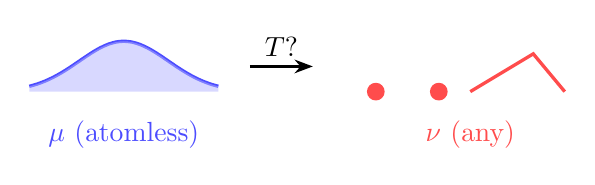
\begin{tikzpicture}[scale=0.8]
    % Source measure (continuous)
    \draw[blue!70, very thick] plot[smooth, domain=0:3] (\x, {0.8*exp(-(\x-1.5)^2)});
    \fill[blue!30, opacity=0.5] plot[smooth, domain=0:3] (\x, {0.8*exp(-(\x-1.5)^2)}) -- (3,0) -- (0,0) -- cycle;
    \node[blue!70, below] at (1.5, -0.3) {$\mu$ (atomless)};

    \draw[-{Stealth}, thick] (3.5, 0.4) -- node[above] {$T$?} (4.5, 0.4);

    % Target measure (any)
    \fill[red!70] (5.5, 0) circle (4pt);
    \fill[red!70] (6.5, 0) circle (4pt);
    \draw[red!70, very thick] (7, 0) -- (8, 0.6) -- (8.5, 0);
    \node[red!70, below] at (7, -0.3) {$\nu$ (any)};
\end{tikzpicture}
\end{center}
\end{frame}

%==============================================================================
\begin{frame}{Lemma 1.27: Existence in 1D}
\begin{block}{Lemma 1.27}
If $\mu, \nu \in \Pp(\R)$ and $\mu$ is \textbf{atomless}, then there exists a transport map $T$ such that $T_\# \mu = \nu$.
\end{block}

\vspace{0.3cm}
\textbf{Proof idea:} Use the \textbf{monotone increasing rearrangement}.

\vspace{0.2cm}
Define CDFs:
\[
F_\mu(x) = \mu((-\infty, x]), \quad F_\nu(y) = \nu((-\infty, y])
\]

\vspace{0.2cm}
The transport map is:
\[
\boxed{T = F_\nu^{-1} \circ F_\mu}
\]

where $F_\nu^{-1}(t) = \inf\{y : F_\nu(y) \geq t\}$ (generalized inverse).

\vspace{0.3cm}
\textbf{Remark:} This map also \textbf{optimizes} the quadratic cost! (Chapter 2)
\end{frame}

%==============================================================================
\begin{frame}{Visualizing 1D Transport}
\begin{center}
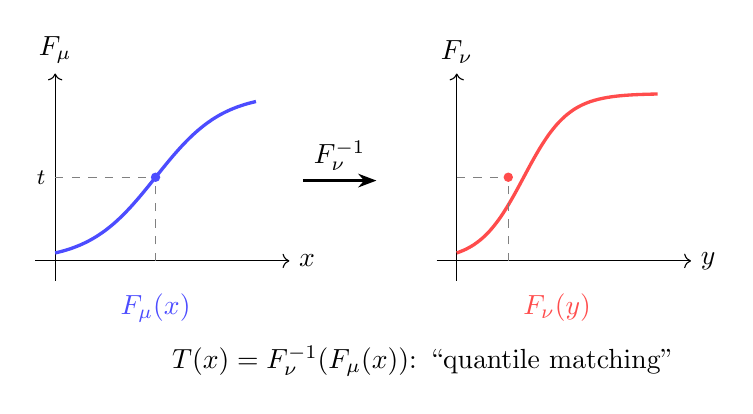
\begin{tikzpicture}[scale=0.85]
    % Left: CDF of mu
    \begin{scope}[shift={(-4,0)}]
        \draw[->] (-0.3,0) -- (3.5,0) node[right] {$x$};
        \draw[->] (0,-0.3) -- (0,2.8) node[above] {$F_\mu$};
        \draw[blue!70, very thick] plot[smooth, domain=0:3] (\x, {2.5*(1/(1+exp(-2*(\x-1.5))))});
        \node[blue!70] at (1.5, -0.7) {$F_\mu(x)$};

        % Horizontal line at 0.5
        \draw[dashed, gray] (0, 1.25) -- (1.5, 1.25);
        \draw[dashed, gray] (1.5, 0) -- (1.5, 1.25);
        \node[left, font=\footnotesize] at (0, 1.25) {$t$};
        \fill[blue!70] (1.5, 1.25) circle (2pt);
    \end{scope}

    % Middle: Arrow
    \draw[-{Stealth}, thick] (-0.3, 1.2) -- node[above] {$F_\nu^{-1}$} (0.8, 1.2);

    % Right: CDF of nu
    \begin{scope}[shift={(2,0)}]
        \draw[->] (-0.3,0) -- (3.5,0) node[right] {$y$};
        \draw[->] (0,-0.3) -- (0,2.8) node[above] {$F_\nu$};
        \draw[red!70, very thick] plot[smooth, domain=0:3] (\x, {2.5*(1/(1+exp(-3*(\x-1))))});
        \node[red!70] at (1.5, -0.7) {$F_\nu(y)$};

        % Horizontal line at 0.5
        \draw[dashed, gray] (0, 1.25) -- (0.77, 1.25);
        \draw[dashed, gray] (0.77, 0) -- (0.77, 1.25);
        \fill[red!70] (0.77, 1.25) circle (2pt);
    \end{scope}

    % Bottom explanation
    \node at (1.5, -1.5) {$T(x) = F_\nu^{-1}(F_\mu(x))$: ``quantile matching''};
\end{tikzpicture}
\end{center}

\vspace{0.2cm}
\textbf{Key insight:} Match quantiles! The point at quantile $t$ in $\mu$ maps to the point at quantile $t$ in $\nu$.
\end{frame}

%==============================================================================
\begin{frame}{Exercise: 1D Transport Construction}
\begin{block}{Exercise}
Let $\mu = \text{Unif}[0,1]$ and $\nu = \text{Unif}[1,3]$.
\begin{enumerate}
    \item[(a)] Find the CDFs $F_\mu$ and $F_\nu$.
    \item[(b)] Compute $T = F_\nu^{-1} \circ F_\mu$ explicitly.
    \item[(c)] Verify that $T_\# \mu = \nu$.
\end{enumerate}
\end{block}

\vspace{0.3cm}
\begin{center}
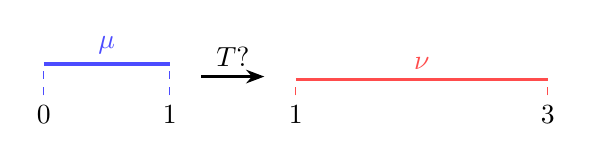
\begin{tikzpicture}[scale=0.8]
    % Source
    \draw[blue!70, very thick] (0, 0.5) -- (2, 0.5);
    \draw[blue!70, dashed] (0, 0) -- (0, 0.5);
    \draw[blue!70, dashed] (2, 0) -- (2, 0.5);
    \node[below] at (0, 0) {$0$};
    \node[below] at (2, 0) {$1$};
    \node[blue!70, above] at (1, 0.5) {$\mu$};

    \draw[-{Stealth}, thick] (2.5, 0.3) -- node[above] {$T$?} (3.5, 0.3);

    % Target
    \draw[red!70, very thick] (4, 0.25) -- (8, 0.25);
    \draw[red!70, dashed] (4, 0) -- (4, 0.25);
    \draw[red!70, dashed] (8, 0) -- (8, 0.25);
    \node[below] at (4, 0) {$1$};
    \node[below] at (8, 0) {$3$};
    \node[red!70, above] at (6, 0.25) {$\nu$};
\end{tikzpicture}
\end{center}
\end{frame}

%==============================================================================
\begin{frame}{Solution: 1D Transport Construction}
\begin{columns}
\begin{column}{0.55\textwidth}
\textbf{(a)} CDFs:
\[
F_\mu(x) = \begin{cases} 0 & x < 0 \\ x & 0 \leq x \leq 1 \\ 1 & x > 1 \end{cases}
\]
\[
F_\nu(y) = \begin{cases} 0 & y < 1 \\ \frac{y-1}{2} & 1 \leq y \leq 3 \\ 1 & y > 3 \end{cases}
\]

\textbf{(b)} Inverse: $F_\nu^{-1}(t) = 2t + 1$

Transport: $\boxed{T(x) = 2x + 1}$

\textbf{(c)} Verification:
\[
T_\# \text{Unif}[0,1] = \text{Unif}[1, 3] = \nu \; \checkmark
\]
\end{column}
\begin{column}{0.45\textwidth}
\begin{center}
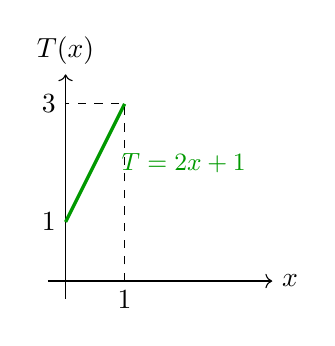
\begin{tikzpicture}[scale=0.75]
    \draw[->] (-0.3, 0) -- (3.5, 0) node[right] {$x$};
    \draw[->] (0, -0.3) -- (0, 3.5) node[above] {$T(x)$};
    \draw[green!60!black, very thick] (0, 1) -- (1, 3);
    \node[below] at (1, 0) {$1$};
    \node[left] at (0, 1) {$1$};
    \node[left] at (0, 3) {$3$};
    \draw[dashed] (1, 0) -- (1, 3) -- (0, 3);
    \node[green!60!black, font=\small] at (2, 2) {$T = 2x + 1$};
\end{tikzpicture}
\end{center}
\end{column}
\end{columns}
\end{frame}

%==============================================================================
\section{From $\R$ to $\R^d$}
%==============================================================================

\begin{frame}{Challenge: Higher Dimensions}
\textbf{In 1D:} Monotone rearrangement works perfectly.

\vspace{0.3cm}
\textbf{In $\R^d$:} No natural ordering!
\begin{itemize}
    \item Which point is ``smaller''? $(1, 2)$ or $(2, 1)$?
    \item Cannot directly define monotone maps
\end{itemize}

\vspace{0.4cm}
\textbf{Clever idea:} Reduce $\R^d$ to $\R$ via a \textbf{bijection}!

\begin{center}
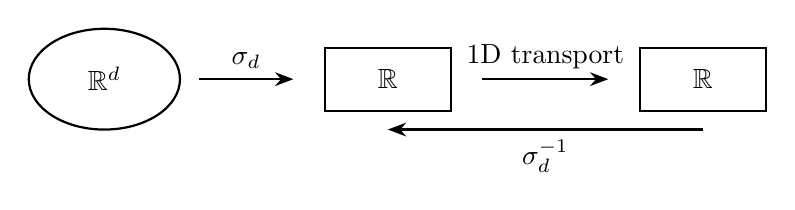
\begin{tikzpicture}[scale=0.8]
    % R^d
    \draw[thick] (0,0) ellipse (1.2 and 0.8);
    \node at (0, 0) {$\R^d$};

    % Arrow to R
    \draw[-{Stealth}, thick] (1.5, 0) -- node[above] {$\sigma_d$} (3, 0);

    % R
    \draw[thick] (3.5, -0.5) -- (5.5, -0.5) -- (5.5, 0.5) -- (3.5, 0.5) -- cycle;
    \node at (4.5, 0) {$\R$};

    % Arrow to R
    \draw[-{Stealth}, thick] (6, 0) -- node[above] {1D transport} (8, 0);

    % R again
    \draw[thick] (8.5, -0.5) -- (10.5, -0.5) -- (10.5, 0.5) -- (8.5, 0.5) -- cycle;
    \node at (9.5, 0) {$\R$};

    % Arrow back
    \draw[-{Stealth}, thick] (9.5, -0.8) -- node[below] {$\sigma_d^{-1}$} (4.5, -0.8);
\end{tikzpicture}
\end{center}
\end{frame}

%==============================================================================
\begin{frame}{Lemma 1.28: Borel Bijection $\sigma_d$}
\begin{block}{Lemma 1.28}
There exists a Borel map $\sigma_d : \R^d \to \R$ which is:
\begin{itemize}
    \item \textbf{Injective}
    \item Its image is a \textbf{Borel subset} of $\R$
    \item Its inverse map is \textbf{Borel measurable}
\end{itemize}
\end{block}

\vspace{0.4cm}
\textbf{Proof strategy:}
\begin{enumerate}
    \item Sufficient to prove for $d = 2$ (then use induction)
    \item Sufficient to work on $]0,1[^2$ (use $\arctan$ to map $\R^2 \to ]0,1[^2$)
    \item Use \textbf{decimal digit interleaving}
\end{enumerate}
\end{frame}

%==============================================================================
\begin{frame}{Proof Step 1: Induction Structure}
\textbf{Induction:} If $\sigma_{d-1} : \R^{d-1} \to \R$ exists, define:
\[
\sigma_d(x_1, x_2, \ldots, x_d) = \sigma_2(x_1, \sigma_{d-1}(x_2, x_3, \ldots, x_d))
\]

\begin{center}
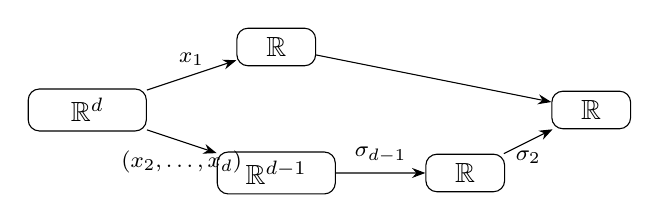
\begin{tikzpicture}[scale=0.8]
    % R^d
    \node[draw, rounded corners, minimum width=1.5cm] (Rd) at (0, 0) {$\R^d$};

    % Split
    \node[draw, rounded corners, minimum width=1cm] (R1) at (3, 1) {$\R$};
    \node[draw, rounded corners, minimum width=1.5cm] (Rd1) at (3, -1) {$\R^{d-1}$};

    % R from R^{d-1}
    \node[draw, rounded corners, minimum width=1cm] (R2) at (6, -1) {$\R$};

    % Final R
    \node[draw, rounded corners, minimum width=1cm] (R) at (8, 0) {$\R$};

    % Arrows
    \draw[-{Stealth}] (Rd) -- node[above, font=\footnotesize] {$x_1$} (R1);
    \draw[-{Stealth}] (Rd) -- node[below, font=\footnotesize] {$(x_2,\ldots,x_d)$} (Rd1);
    \draw[-{Stealth}] (Rd1) -- node[above, font=\footnotesize] {$\sigma_{d-1}$} (R2);
    \draw[-{Stealth}] (R1) -- (R);
    \draw[-{Stealth}] (R2) -- node[below, font=\footnotesize] {$\sigma_2$} (R);
\end{tikzpicture}
\end{center}

\vspace{0.2cm}
$\Rightarrow$ Only need to construct $\sigma_2$!
\end{frame}

%==============================================================================
\begin{frame}{Proof Step 2: Reduce to $]0,1[^2$}
\textbf{Map $\R^2$ to $]0,1[^2$:}
\[
(x, y) \mapsto \left(\frac{1}{2} + \frac{1}{\pi}\arctan(x), \; \frac{1}{2} + \frac{1}{\pi}\arctan(y)\right)
\]

This is a \textbf{bijection} $\R^2 \leftrightarrow ]0,1[^2$.

\begin{center}
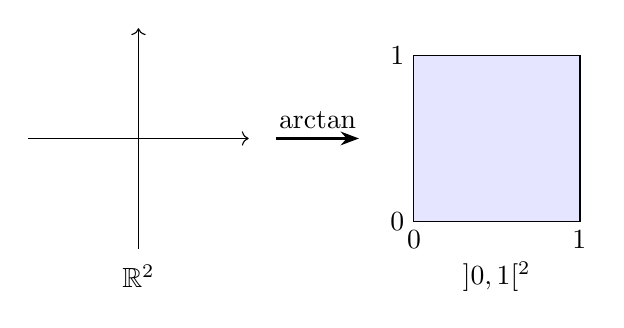
\begin{tikzpicture}[scale=0.7]
    % R^2
    \draw[->] (-2, 0) -- (2, 0);
    \draw[->] (0, -2) -- (0, 2);
    \node at (0, -2.5) {$\R^2$};

    \draw[-{Stealth}, thick] (2.5, 0) -- node[above] {$\arctan$} (4, 0);

    % ]0,1[^2
    \draw[thick] (5, -1.5) rectangle (8, 1.5);
    \node[below] at (5, -1.5) {$0$};
    \node[below] at (8, -1.5) {$1$};
    \node[left] at (5, -1.5) {$0$};
    \node[left] at (5, 1.5) {$1$};
    \node at (6.5, -2.5) {$]0,1[^2$};

    % Shading
    \fill[blue!10] (5, -1.5) rectangle (8, 1.5);
\end{tikzpicture}
\end{center}

\vspace{0.2cm}
$\Rightarrow$ Only need to construct $\sigma_2 : ]0,1[^2 \to ]0,1[$!
\end{frame}

%==============================================================================
\begin{frame}{The Decimal Interleaving Map}
\textbf{Construction:} For $(x, y) \in ]0,1[^2$ with decimal expansions:
\[
x = 0.x_1 x_2 x_3 \ldots, \quad y = 0.y_1 y_2 y_3 \ldots
\]

\textbf{Define:}
\[
\boxed{\sigma_2(x, y) = 0.x_1 y_1 x_2 y_2 x_3 y_3 \ldots}
\]

\begin{center}
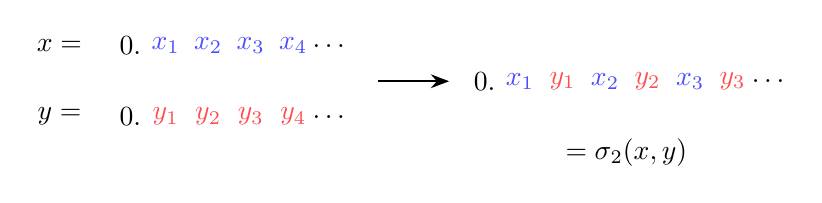
\begin{tikzpicture}[scale=0.9]
    % x digits
    \node at (-1, 1) {$x =$};
    \node at (0, 1) {$0.$};
    \node[blue!70, font=\bfseries] at (0.5, 1) {$x_1$};
    \node[blue!70, font=\bfseries] at (1.1, 1) {$x_2$};
    \node[blue!70, font=\bfseries] at (1.7, 1) {$x_3$};
    \node[blue!70, font=\bfseries] at (2.3, 1) {$x_4$};
    \node at (2.8, 1) {$\ldots$};

    % y digits
    \node at (-1, 0) {$y =$};
    \node at (0, 0) {$0.$};
    \node[red!70, font=\bfseries] at (0.5, 0) {$y_1$};
    \node[red!70, font=\bfseries] at (1.1, 0) {$y_2$};
    \node[red!70, font=\bfseries] at (1.7, 0) {$y_3$};
    \node[red!70, font=\bfseries] at (2.3, 0) {$y_4$};
    \node at (2.8, 0) {$\ldots$};

    % Arrow
    \draw[-{Stealth}, thick] (3.5, 0.5) -- (4.5, 0.5);

    % Result
    \node at (5, 0.5) {$0.$};
    \node[blue!70, font=\bfseries] at (5.5, 0.5) {$x_1$};
    \node[red!70, font=\bfseries] at (6.1, 0.5) {$y_1$};
    \node[blue!70, font=\bfseries] at (6.7, 0.5) {$x_2$};
    \node[red!70, font=\bfseries] at (7.3, 0.5) {$y_2$};
    \node[blue!70, font=\bfseries] at (7.9, 0.5) {$x_3$};
    \node[red!70, font=\bfseries] at (8.5, 0.5) {$y_3$};
    \node at (9, 0.5) {$\ldots$};

    \node at (7, -0.5) {$= \sigma_2(x, y)$};
\end{tikzpicture}
\end{center}

\vspace{0.2cm}
\textbf{Convention:} No decimal ending in periodic $9$ (e.g., $0.3472\overline{9} \to 0.3473$).
\end{frame}

%==============================================================================
\begin{frame}{Example: Decimal Interleaving}
\textbf{Example:}
\begin{align*}
x &= 0.314159\ldots \quad (\approx \pi/10) \\
y &= 0.271828\ldots \quad (\approx e/10)
\end{align*}

\textbf{Interleaving:}
\[
\sigma_2(x, y) = 0.\textcolor{blue!70}{3}\textcolor{red!70}{2}\textcolor{blue!70}{1}\textcolor{red!70}{7}\textcolor{blue!70}{4}\textcolor{red!70}{1}\textcolor{blue!70}{1}\textcolor{red!70}{8}\textcolor{blue!70}{5}\textcolor{red!70}{2}\textcolor{blue!70}{9}\textcolor{red!70}{8}\ldots = 0.327141185298\ldots
\]

\begin{center}
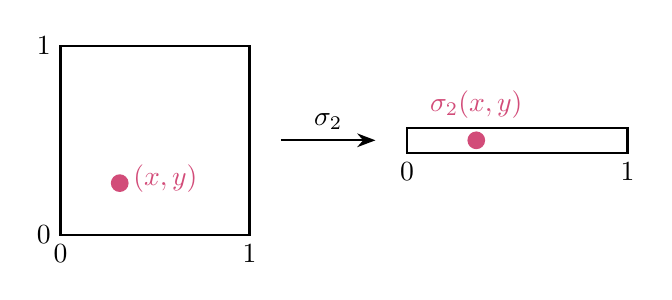
\begin{tikzpicture}[scale=0.8]
    % Unit square
    \draw[thick] (0, 0) rectangle (3, 3);
    \node[below] at (0, 0) {$0$};
    \node[below] at (3, 0) {$1$};
    \node[left] at (0, 0) {$0$};
    \node[left] at (0, 3) {$1$};

    % Point (x, y)
    \fill[purple!70] (0.94, 0.82) circle (4pt);
    \node[right, purple!70] at (1, 0.9) {$(x, y)$};

    % Arrow
    \draw[-{Stealth}, thick] (3.5, 1.5) -- node[above] {$\sigma_2$} (5, 1.5);

    % Unit interval
    \draw[thick] (5.5, 1.3) -- (9, 1.3) -- (9, 1.7) -- (5.5, 1.7) -- cycle;
    \node[below] at (5.5, 1.3) {$0$};
    \node[below] at (9, 1.3) {$1$};

    % Point sigma_2(x,y)
    \fill[purple!70] (6.6, 1.5) circle (4pt);
    \node[above, purple!70] at (6.6, 1.7) {$\sigma_2(x,y)$};
\end{tikzpicture}
\end{center}
\end{frame}

%==============================================================================
\begin{frame}{Exercise: Interleaving Computation}
\begin{block}{Exercise}
Compute $\sigma_2$ and $\sigma_2^{-1}$:
\begin{enumerate}
    \item[(a)] $\sigma_2(0.25, 0.50) = ?$
    \item[(b)] $\sigma_2^{-1}(0.1234) = ?$
    \item[(c)] Why is $0.393939\ldots$ (periodic) \textbf{not} in the image of $\sigma_2$?
\end{enumerate}
\end{block}

\vspace{0.4cm}
\textit{Hint for (c):} What would the preimage be?
\end{frame}

%==============================================================================
\begin{frame}{Solution: Interleaving Computation}
\textbf{(a)} $\sigma_2(0.25, 0.50)$:
\begin{itemize}
    \item $0.25 = 0.2500\ldots$, \quad $0.50 = 0.5000\ldots$
    \item $\sigma_2(0.25, 0.50) = 0.\textcolor{blue!70}{2}\textcolor{red!70}{5}\textcolor{blue!70}{5}\textcolor{red!70}{0}\textcolor{blue!70}{0}\textcolor{red!70}{0}\ldots = \boxed{0.255}$
\end{itemize}

\vspace{0.3cm}
\textbf{(b)} $\sigma_2^{-1}(0.1234)$:
\begin{itemize}
    \item $0.1234 = 0.12340000\ldots$
    \item Extract odd positions: $x = 0.1300\ldots = 0.13$
    \item Extract even positions: $y = 0.2400\ldots = 0.24$
    \item $\sigma_2^{-1}(0.1234) = \boxed{(0.13, 0.24)}$
\end{itemize}

\vspace{0.3cm}
\textbf{(c)} $0.\overline{39} = 0.393939\ldots$:
\begin{itemize}
    \item If $\sigma_2(x, y) = 0.\overline{39}$, then $x = 0.333\ldots = 0.\overline{3}$ and $y = 0.999\ldots = 0.\overline{9}$
    \item But $0.\overline{9} = 1 \notin ]0,1[$!
    \item We \textbf{forbid} decimals ending in periodic $9$ $\Rightarrow$ $0.\overline{39}$ is not in the image.
\end{itemize}
\end{frame}

%==============================================================================
\begin{frame}{Measurability of $\sigma_2$}
\textbf{Why is $\sigma_2$ Borel measurable?}

\vspace{0.3cm}
Consider an interval in $\R$ defined by first $2k$ digits:
\[
I = [0.a_1b_1a_2b_2\ldots a_kb_k, \; 0.a_1b_1a_2b_2\ldots a_kb_k + 10^{-2k}]
\]

\textbf{Preimage:}
\[
\sigma_2^{-1}(I) = [0.a_1a_2\ldots a_k, 0.a_1a_2\ldots a_k + 10^{-k}] \times [0.b_1b_2\ldots b_k, 0.b_1b_2\ldots b_k + 10^{-k}]
\]

This is a \textbf{rectangle} in $\R^2$!

\begin{center}
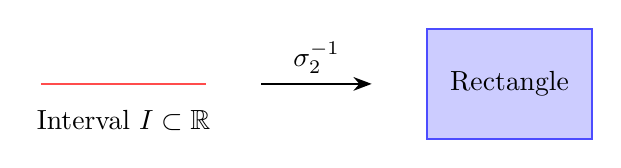
\begin{tikzpicture}[scale=0.7]
    % Interval
    \draw[thick, red!70] (0, 0) -- (3, 0);
    \node[below] at (1.5, -0.3) {Interval $I \subset \R$};

    \draw[-{Stealth}, thick] (4, 0) -- node[above] {$\sigma_2^{-1}$} (6, 0);

    % Rectangle
    \fill[blue!20] (7, -1) rectangle (10, 1);
    \draw[thick, blue!70] (7, -1) rectangle (10, 1);
    \node at (8.5, 0) {Rectangle};
\end{tikzpicture}
\end{center}

These intervals generate the Borel $\sigma$-algebra $\Rightarrow$ $\sigma_2$ is Borel measurable.
\end{frame}

%==============================================================================
\begin{frame}{Corollary 1.29: Transport Maps in $\R^d$}
\begin{block}{Corollary 1.29}
If $\mu, \nu \in \Pp(\R^d)$ and $\mu$ is \textbf{atomless}, then there exists a transport map $T$ such that $T_\# \mu = \nu$.
\end{block}

\vspace{0.3cm}
\textbf{Proof:}
\begin{enumerate}
    \item Push $\mu, \nu$ to $\R$ via $\sigma_d$: get $(\sigma_d)_\# \mu$ and $(\sigma_d)_\# \nu$
    \item $(\sigma_d)_\# \mu$ is atomless (since $\sigma_d$ is injective)
    \item By Lemma 1.27: $\exists$ transport $S : \R \to \R$ with $S_\# ((\sigma_d)_\# \mu) = (\sigma_d)_\# \nu$
    \item Define: $T = \sigma_d^{-1} \circ S \circ \sigma_d$
\end{enumerate}

\begin{center}
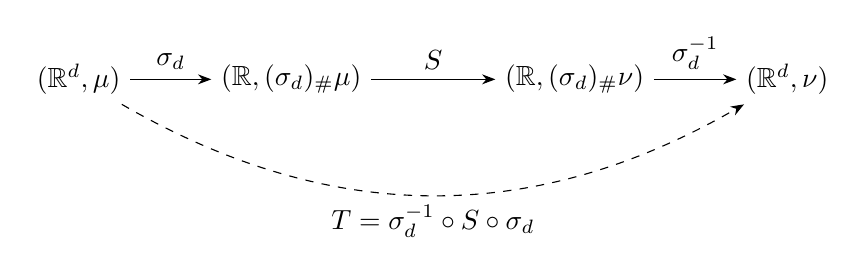
\begin{tikzpicture}[scale=0.9]
    \node (Rd1) at (0, 0) {$(\R^d, \mu)$};
    \node (R1) at (3, 0) {$(\R, (\sigma_d)_\# \mu)$};
    \node (R2) at (7, 0) {$(\R, (\sigma_d)_\# \nu)$};
    \node (Rd2) at (10, 0) {$(\R^d, \nu)$};

    \draw[-{Stealth}] (Rd1) -- node[above] {$\sigma_d$} (R1);
    \draw[-{Stealth}] (R1) -- node[above] {$S$} (R2);
    \draw[-{Stealth}] (R2) -- node[above] {$\sigma_d^{-1}$} (Rd2);
    \draw[-{Stealth}, dashed, bend right=30] (Rd1) to node[below] {$T = \sigma_d^{-1} \circ S \circ \sigma_d$} (Rd2);
\end{tikzpicture}
\end{center}
\end{frame}

%==============================================================================
\begin{frame}{Exercise: Transport to a Dirac Mass}
\begin{block}{Exercise}
Let $\mu = \text{Unif}([0,1]^2)$ (Lebesgue measure on unit square) and $\nu = \delta_{(0.5, 0.5)}$.
\begin{enumerate}
    \item[(a)] Is $\mu$ atomless? Is $\nu$ atomless?
    \item[(b)] Does Corollary 1.29 guarantee a transport $T$ with $T_\# \mu = \nu$?
    \item[(c)] Can you describe such a $T$ explicitly?
\end{enumerate}
\end{block}

\begin{center}
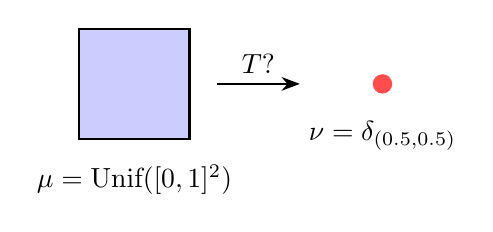
\begin{tikzpicture}[scale=0.7]
    % Unit square with shading
    \fill[blue!20] (0, 0) rectangle (2, 2);
    \draw[thick] (0, 0) rectangle (2, 2);
    \node[below] at (1, -0.3) {$\mu = \text{Unif}([0,1]^2)$};

    \draw[-{Stealth}, thick] (2.5, 1) -- node[above] {$T$?} (4, 1);

    % Single point
    \fill[red!70] (5.5, 1) circle (5pt);
    \node[below] at (5.5, 0.5) {$\nu = \delta_{(0.5, 0.5)}$};
\end{tikzpicture}
\end{center}
\end{frame}

%==============================================================================
\begin{frame}{Solution: Transport to a Dirac Mass}
\textbf{(a)}
\begin{itemize}
    \item $\mu$ is \textbf{atomless} (Lebesgue measure on $[0,1]^2$)
    \item $\nu$ is \textbf{atomic} (single point mass at $(0.5, 0.5)$)
\end{itemize}

\vspace{0.3cm}
\textbf{(b)} \textbf{Yes!} Corollary 1.29 only requires $\mu$ to be atomless.

\vspace{0.3cm}
\textbf{(c)} The transport map is simply:
\[
\boxed{T(x, y) = (0.5, 0.5) \quad \text{for all } (x, y) \in [0,1]^2}
\]

This is a \textbf{constant map}! It sends all mass to the single atom.

\begin{center}
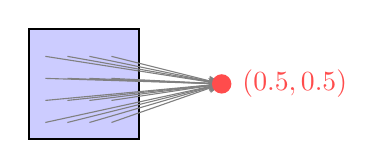
\begin{tikzpicture}[scale=0.7]
    % Unit square with arrows
    \fill[blue!20] (0, 0) rectangle (2, 2);
    \draw[thick] (0, 0) rectangle (2, 2);

    \foreach \x in {0.3, 0.7, 1.1, 1.5} {
        \foreach \y in {0.3, 0.7, 1.1, 1.5} {
            \draw[-{Stealth}, gray, thin] (\x, \y) -- (3.5, 1);
        }
    }

    % Target
    \fill[red!70] (3.5, 1) circle (5pt);
    \node[right, red!70] at (3.7, 1) {$(0.5, 0.5)$};
\end{tikzpicture}
\end{center}

Verification: $T_\# \mu(\{(0.5, 0.5)\}) = \mu(T^{-1}(\{(0.5, 0.5)\})) = \mu([0,1]^2) = 1$ \checkmark
\end{frame}

%==============================================================================
\section{Weak Convergence from Partitions}
%==============================================================================

\begin{frame}{Setup: Partition Convergence}
\textbf{Setting:}
\begin{itemize}
    \item $X$: compact metric space
    \item $\rho \in \Pp(X)$: probability measure
    \item $\mathcal{G}_n$: partition of $X$ into sets $C_{i,n}$ for $i \in I_n$
    \item $\text{size}(\mathcal{G}_n) := \max_i \text{diam}(C_{i,n}) \to 0$ as $n \to \infty$
\end{itemize}

\begin{center}
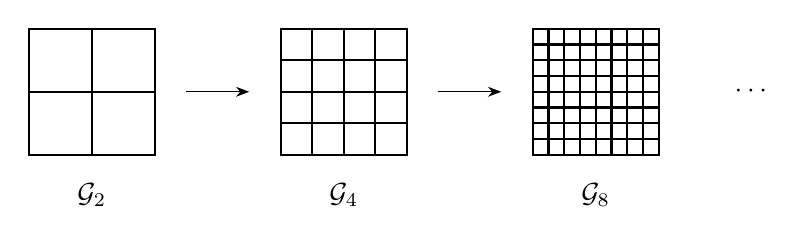
\begin{tikzpicture}[scale=0.8]
    % Coarse partition (n=2)
    \begin{scope}[shift={(-3, 0)}]
        \draw[thick] (0, 0) rectangle (2, 2);
        \draw[thick] (1, 0) -- (1, 2);
        \draw[thick] (0, 1) -- (2, 1);
        \node[below] at (1, -0.3) {$\mathcal{G}_2$};
    \end{scope}

    % Arrow
    \draw[-{Stealth}] (-0.5, 1) -- (0.5, 1);

    % Finer partition (n=4)
    \begin{scope}[shift={(1, 0)}]
        \draw[thick] (0, 0) rectangle (2, 2);
        \foreach \x in {0.5, 1, 1.5} {
            \draw[thick] (\x, 0) -- (\x, 2);
        }
        \foreach \y in {0.5, 1, 1.5} {
            \draw[thick] (0, \y) -- (2, \y);
        }
        \node[below] at (1, -0.3) {$\mathcal{G}_4$};
    \end{scope}

    % Arrow
    \draw[-{Stealth}] (3.5, 1) -- (4.5, 1);

    % Even finer
    \begin{scope}[shift={(5, 0)}]
        \draw[thick] (0, 0) rectangle (2, 2);
        \foreach \x in {0.25, 0.5, ..., 1.75} {
            \draw[thick] (\x, 0) -- (\x, 2);
        }
        \foreach \y in {0.25, 0.5, ..., 1.75} {
            \draw[thick] (0, \y) -- (2, \y);
        }
        \node[below] at (1, -0.3) {$\mathcal{G}_8$};
    \end{scope}

    \node at (8.5, 1) {$\cdots$};
\end{tikzpicture}
\end{center}

\textbf{Question:} If $\rho_n$ has the \textbf{same mass} as $\rho$ on each cell, does $\rho_n \rightharpoonup \rho$?
\end{frame}

%==============================================================================
\begin{frame}{Lemma 1.31: Weak Convergence from Partitions}
\begin{block}{Lemma 1.31}
If $\rho_n \in \Pp(X)$ satisfies $\rho_n(C_{i,n}) = \rho(C_{i,n})$ for all $i \in I_n$ and all $n$, then:
\[
\rho_n \rightharpoonup \rho \quad \text{(weakly)}
\]
\end{block}

\vspace{0.3cm}
\textbf{Key idea:} Same mass on each partition cell + small cells $\Rightarrow$ integrals converge.

\begin{center}
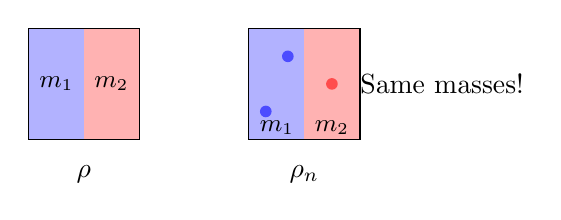
\begin{tikzpicture}[scale=0.7]
    % rho
    \begin{scope}[shift={(-3, 0)}]
        \draw[thick] (0, 0) rectangle (2, 2);
        \draw[thick] (1, 0) -- (1, 2);
        \fill[blue!30] (0, 0) rectangle (1, 2);
        \fill[red!30] (1, 0) rectangle (2, 2);
        \node[font=\small] at (0.5, 1) {$m_1$};
        \node[font=\small] at (1.5, 1) {$m_2$};
        \node[below] at (1, -0.3) {$\rho$};
    \end{scope}

    % rho_n
    \begin{scope}[shift={(1, 0)}]
        \draw[thick] (0, 0) rectangle (2, 2);
        \draw[thick] (1, 0) -- (1, 2);
        \fill[blue!30] (0, 0) rectangle (1, 2);
        \fill[red!30] (1, 0) rectangle (2, 2);
        % Different internal distribution
        \fill[blue!70] (0.3, 0.5) circle (3pt);
        \fill[blue!70] (0.7, 1.5) circle (3pt);
        \fill[red!70] (1.5, 1) circle (3pt);
        \node[font=\small] at (0.5, 0.2) {$m_1$};
        \node[font=\small] at (1.5, 0.2) {$m_2$};
        \node[below] at (1, -0.3) {$\rho_n$};
    \end{scope}

    \node at (4.5, 1) {Same masses!};
\end{tikzpicture}
\end{center}
\end{frame}

%==============================================================================
\begin{frame}{Proof of Lemma 1.31}
Let $\phi \in C(X)$ with modulus of continuity $\omega$. Set $m_{i,n} := \rho_n(C_{i,n}) = \rho(C_{i,n})$.

\vspace{0.2cm}
\textbf{Estimate:}
\[
\left| \int_X \phi \, d\rho_n - \int_X \phi \, d\rho \right| \leq \sum_{i \in I_n} \left| \int_{C_{i,n}} \phi \, d\rho_n - \int_{C_{i,n}} \phi \, d\rho \right|
\]

On each cell $C_{i,n}$, the oscillation of $\phi$ is at most $\omega(\text{diam}(C_{i,n}))$.

Since $\rho_n(C_{i,n}) = \rho(C_{i,n}) = m_{i,n}$:
\[
\left| \int_{C_{i,n}} \phi \, d\rho_n - \int_{C_{i,n}} \phi \, d\rho \right| \leq \omega(\text{diam}(C_{i,n})) \cdot m_{i,n}
\]

\textbf{Sum:} $\displaystyle \leq \omega(\text{size}(\mathcal{G}_n)) \sum_{i} m_{i,n} = \omega(\text{size}(\mathcal{G}_n)) \to 0$ as $n \to \infty$. \hfill $\square$
\end{frame}

%==============================================================================
\begin{frame}{Exercise: Partition Convergence}
\begin{block}{Exercise}
Let $X = [0,1]$, $\rho = \text{Unif}[0,1]$.

Partition: $\mathcal{G}_n$ with $C_{i,n} = \left[\frac{i-1}{n}, \frac{i}{n}\right]$ for $i = 1, \ldots, n$.

Define $\rho_n = \frac{1}{n} \sum_{i=1}^{n} \delta_{\frac{2i-1}{2n}}$ (Dirac masses at midpoints).
\begin{enumerate}
    \item[(a)] Verify that $\rho_n(C_{i,n}) = \rho(C_{i,n})$ for all $i$.
    \item[(b)] Compute $\int_0^1 x \, d\rho_n$ and $\int_0^1 x \, d\rho$.
    \item[(c)] For general $\phi \in C([0,1])$, show $\left|\int \phi \, d\rho_n - \int \phi \, d\rho\right| \leq \omega(1/n)$.
\end{enumerate}
\end{block}

\begin{center}
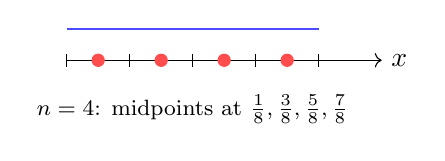
\begin{tikzpicture}[scale=0.8]
    \draw[->] (0, 0) -- (5, 0) node[right] {$x$};
    \draw[thick, blue!70] (0, 0.5) -- (4, 0.5);

    % Partition marks
    \foreach \i in {0, 1, 2, 3, 4} {
        \draw (\i, -0.1) -- (\i, 0.1);
    }

    % Midpoint masses
    \foreach \i in {0.5, 1.5, 2.5, 3.5} {
        \fill[red!70] (\i, 0) circle (3pt);
    }

    \node[below, font=\footnotesize] at (2, -0.4) {$n = 4$: midpoints at $\frac{1}{8}, \frac{3}{8}, \frac{5}{8}, \frac{7}{8}$};
\end{tikzpicture}
\end{center}
\end{frame}

%==============================================================================
\begin{frame}{Solution: Partition Convergence}
\textbf{(a)} Each cell $C_{i,n} = \left[\frac{i-1}{n}, \frac{i}{n}\right]$ contains exactly one midpoint $\frac{2i-1}{2n}$.
\[
\rho_n(C_{i,n}) = \frac{1}{n}, \quad \rho(C_{i,n}) = \frac{1}{n} \quad \checkmark
\]

\vspace{0.3cm}
\textbf{(b)}
\[
\int_0^1 x \, d\rho_n = \frac{1}{n} \sum_{i=1}^{n} \frac{2i-1}{2n} = \frac{1}{2n^2} \sum_{i=1}^{n} (2i-1) = \frac{1}{2n^2} \cdot n^2 = \boxed{\frac{1}{2}}
\]
\[
\int_0^1 x \, d\rho = \frac{1}{2} \quad \checkmark \quad \text{(Already equal!)}
\]

\vspace{0.3cm}
\textbf{(c)} By the proof of Lemma 1.31:
\[
\left|\int \phi \, d\rho_n - \int \phi \, d\rho\right| \leq \omega\left(\frac{1}{n}\right) \to 0
\]
where $\omega$ is the modulus of continuity of $\phi$.
\end{frame}

%==============================================================================
\section{Density of Map-Induced Plans}
%==============================================================================

\begin{frame}{The Density Question}
\textbf{Recall:}
\begin{itemize}
    \item $\Pi(\mu, \nu)$: all transport plans (joint measures with marginals $\mu, \nu$)
    \item $\{\gamma_T : T \text{ is a transport map}\}$: map-induced plans (concentrated on graph of $T$)
\end{itemize}

\vspace{0.3cm}
Map-induced plans are a \textbf{subset} of all plans.

\vspace{0.4cm}
\textbf{Question:} How ``big'' is this subset?

\begin{center}
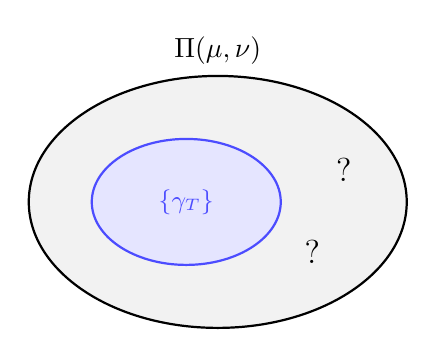
\begin{tikzpicture}[scale=0.8]
    % All plans
    \draw[thick, fill=gray!10] (0, 0) ellipse (3 and 2);
    \node at (0, 2.4) {$\Pi(\mu, \nu)$};

    % Map-induced (subset)
    \draw[thick, blue!70, fill=blue!10] (-0.5, 0) ellipse (1.5 and 1);
    \node[blue!70, font=\small] at (-0.5, 0) {$\{\gamma_T\}$};

    % Question marks
    \node[font=\large] at (2, 0.5) {?};
    \node[font=\large] at (1.5, -0.8) {?};
\end{tikzpicture}
\end{center}
\end{frame}

%==============================================================================
\begin{frame}{Theorem 1.32: Density Result}
\begin{block}{Theorem 1.32}
On a compact subset $\Omega \subset \R^d$, the set of map-induced plans $\gamma_T$ is \textbf{dense} in $\Pi(\mu, \nu)$ (weak topology) whenever $\mu$ is atomless.
\end{block}

\vspace{0.2cm}
\textbf{Remarkable:} Even though map-induced plans are ``special'' (concentrated on a graph), they can \textbf{approximate any plan}!

\begin{center}
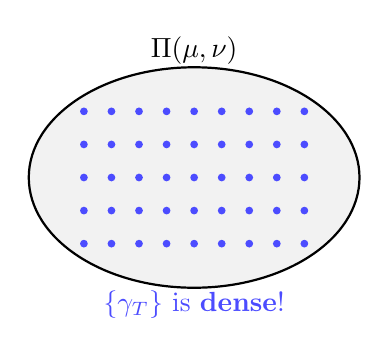
\begin{tikzpicture}[scale=0.7]
    % All plans
    \draw[thick, fill=gray!10] (0, 0) ellipse (3 and 2);
    \node at (0, 2.3) {$\Pi(\mu, \nu)$};

    % Map-induced (dense)
    \foreach \x in {-2, -1.5, -1, -0.5, 0, 0.5, 1, 1.5, 2} {
        \foreach \y in {-1.2, -0.6, 0, 0.6, 1.2} {
            \pgfmathsetmacro{\r}{sqrt(\x*\x/9 + \y*\y/4)}
            \pgfmathparse{\r < 0.95 ? 1 : 0}
            \ifnum\pgfmathresult=1
                \fill[blue!70] (\x, \y) circle (2pt);
            \fi
        }
    }

    \node[blue!70] at (0, -2.3) {$\{\gamma_T\}$ is \textbf{dense}!};
\end{tikzpicture}
\end{center}
\end{frame}

%==============================================================================
\begin{frame}{Proof Setup}
\textbf{Goal:} Given any $\gamma \in \Pi(\mu, \nu)$, find transport maps $T_n$ with $\gamma_{T_n} \rightharpoonup \gamma$.

\vspace{0.3cm}
\textbf{Setup:}
\begin{itemize}
    \item Fix $n$, partition $\Omega$ into sets $K_{i,n}$ with $\text{diam} < \frac{1}{2n}$
    \item Product partition: $C_{i,j,n} := K_{i,n} \times K_{j,n}$
    \item This partitions $\Omega \times \Omega$ with size $< \frac{1}{n}$
\end{itemize}

\begin{center}
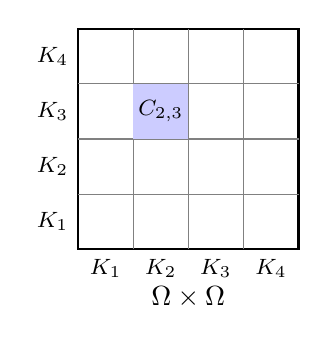
\begin{tikzpicture}[scale=0.7]
    % Grid on Omega x Omega
    \draw[thick] (0, 0) rectangle (4, 4);
    \foreach \x in {1, 2, 3} {
        \draw[gray] (\x, 0) -- (\x, 4);
        \draw[gray] (0, \x) -- (4, \x);
    }

    % Labels
    \node[below] at (0.5, 0) {\footnotesize $K_1$};
    \node[below] at (1.5, 0) {\footnotesize $K_2$};
    \node[below] at (2.5, 0) {\footnotesize $K_3$};
    \node[below] at (3.5, 0) {\footnotesize $K_4$};

    \node[left] at (0, 0.5) {\footnotesize $K_1$};
    \node[left] at (0, 1.5) {\footnotesize $K_2$};
    \node[left] at (0, 2.5) {\footnotesize $K_3$};
    \node[left] at (0, 3.5) {\footnotesize $K_4$};

    % One cell highlighted
    \fill[blue!20] (1, 2) rectangle (2, 3);
    \node[font=\footnotesize] at (1.5, 2.5) {$C_{2,3}$};

    \node[below] at (2, -0.5) {$\Omega \times \Omega$};
\end{tikzpicture}
\end{center}

\textbf{Strategy:} Build $T$ such that $\gamma_T(C_{i,j,n}) = \gamma(C_{i,j,n})$ for all $i, j$.
\end{frame}

%==============================================================================
\begin{frame}{Proof: Column Decomposition}
\textbf{Key idea:} Work column by column!

\vspace{0.2cm}
Define \textbf{columns}: $\text{Col}_{i,n} := K_{i,n} \times \Omega$

\begin{columns}
\begin{column}{0.5\textwidth}
For each column $i$:
\begin{itemize}
    \item $\gamma_{i,n}$ := restriction of $\gamma$ to $\text{Col}_{i,n}$
    \item First marginal: $\mu_{i,n}$ (supported on $K_{i,n}$)
    \item Second marginal: $\nu_{i,n}$
\end{itemize}

\vspace{0.2cm}
\textbf{Crucial:} $\mu_{i,n} \leq \mu$

$\Rightarrow$ $\mu_{i,n}$ is \textbf{atomless}!
\end{column}
\begin{column}{0.5\textwidth}
\begin{center}
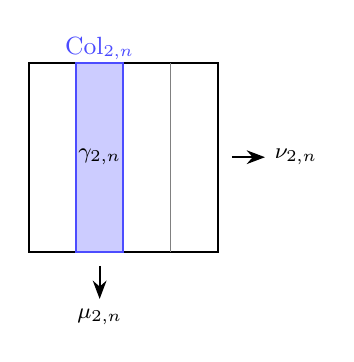
\begin{tikzpicture}[scale=0.6]
    \draw[thick] (0, 0) rectangle (4, 4);
    \foreach \x in {1, 2, 3} {
        \draw[gray] (\x, 0) -- (\x, 4);
    }

    % Highlight column 2
    \fill[blue!20] (1, 0) rectangle (2, 4);
    \draw[thick, blue!70] (1, 0) rectangle (2, 4);

    \node[blue!70, font=\small] at (1.5, 4.3) {$\text{Col}_{2,n}$};
    \node[font=\footnotesize] at (1.5, 2) {$\gamma_{2,n}$};

    % Marginals
    \draw[-{Stealth}, thick] (1.5, -0.3) -- (1.5, -1);
    \node[below, font=\footnotesize] at (1.5, -1) {$\mu_{2,n}$};

    \draw[-{Stealth}, thick] (4.3, 2) -- (5, 2);
    \node[right, font=\footnotesize] at (5, 2) {$\nu_{2,n}$};
\end{tikzpicture}
\end{center}
\end{column}
\end{columns}
\end{frame}

%==============================================================================
\begin{frame}{Proof: Building the Transport}
\textbf{For each column $i$:}
\begin{enumerate}
    \item $\mu_{i,n}$ is atomless (since $\mu_{i,n} \leq \mu$ and $\mu$ is atomless)
    \item By Corollary 1.29: $\exists$ transport $T_{i,n}$ with $(T_{i,n})_\# \mu_{i,n} = \nu_{i,n}$
\end{enumerate}

\vspace{0.3cm}
\textbf{Glue together:}
\[
T(x) = T_{i,n}(x) \quad \text{for } x \in K_{i,n}
\]

\vspace{0.2cm}
\textbf{Check marginals:}
\begin{itemize}
    \item $\sum_i \mu_{i,n} = \mu$ \checkmark
    \item $\sum_i \nu_{i,n} = \nu$ \checkmark
    \item So $T_\# \mu = \nu$ \checkmark
\end{itemize}

\begin{center}
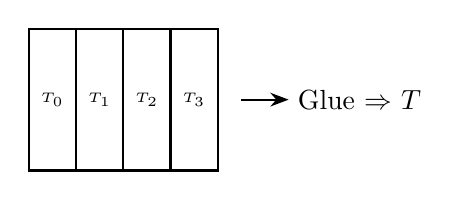
\begin{tikzpicture}[scale=0.6]
    % Columns
    \foreach \i in {0, 1, 2, 3} {
        \draw[thick] (\i, 0) rectangle (\i+1, 3);
        \node[font=\tiny] at (\i+0.5, 1.5) {$T_{\i}$};
    }

    \draw[-{Stealth}, thick] (4.5, 1.5) -- (5.5, 1.5);

    \node at (7, 1.5) {Glue $\Rightarrow$ $T$};
\end{tikzpicture}
\end{center}
\end{frame}

%==============================================================================
\begin{frame}{Proof: Verification}
\textbf{Need to check:} $\gamma_T(C_{i,j,n}) = \gamma(C_{i,j,n})$ for all $i, j$.

\vspace{0.3cm}
For $C_{i,j,n} = K_{i,n} \times K_{j,n}$:
\begin{align*}
\gamma_T(C_{i,j,n}) &= \gamma_{T_{i,n}}(C_{i,j,n}) \\
&= \mu_{i,n}(\{x \in K_{i,n} : T_{i,n}(x) \in K_{j,n}\}) \\
&= \nu_{i,n}(K_{j,n}) \quad \text{(since } (T_{i,n})_\# \mu_{i,n} = \nu_{i,n}\text{)} \\
&= \gamma(K_{i,n} \times K_{j,n}) \\
&= \gamma(C_{i,j,n}) \quad \checkmark
\end{align*}

\vspace{0.3cm}
By Lemma 1.31: $\gamma_{T_n} \rightharpoonup \gamma$ as $n \to \infty$. \hfill $\square$
\end{frame}

%==============================================================================
\begin{frame}{Exercise: Density Approximation}
\begin{block}{Exercise}
Consider $\mu = \nu = \text{Unif}[0,1]$ and $\gamma = \mu \otimes \nu$ (independent coupling).
\begin{enumerate}
    \item[(a)] Is $\gamma$ induced by a transport map?
    \item[(b)] For $n = 2$, construct $T_2$ following the proof of Theorem 1.32.
    \item[(c)] Describe what $\gamma_{T_2}$ looks like.
\end{enumerate}
\end{block}

\begin{center}
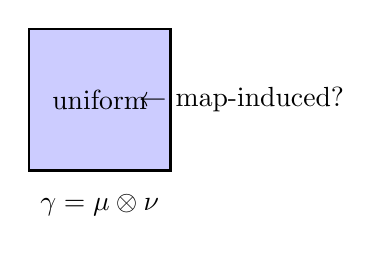
\begin{tikzpicture}[scale=0.6]
    % gamma = mu x nu (spread out)
    \fill[blue!20] (0, 0) rectangle (3, 3);
    \draw[thick] (0, 0) rectangle (3, 3);
    \node[below] at (1.5, -0.3) {$\gamma = \mu \otimes \nu$};
    \node at (1.5, 1.5) {uniform};

    \node at (4.5, 1.5) {$\leftarrow$ map-induced?};
\end{tikzpicture}
\end{center}
\end{frame}

%==============================================================================
\begin{frame}{Solution: Density Approximation}
\textbf{(a)} \textbf{No!} $\gamma = \mu \otimes \nu$ spreads mass uniformly over $[0,1]^2$.

A map-induced plan $\gamma_T$ is concentrated on the graph $\{(x, T(x))\}$ --- a 1D curve!

\vspace{0.3cm}
\textbf{(b)} For $n = 2$: Partition $[0,1]$ into $K_1 = [0, \frac{1}{2}]$, $K_2 = [\frac{1}{2}, 1]$.

For each column:
\begin{itemize}
    \item $\mu_{1,2} = \text{Unif}[0, \frac{1}{2}]$, $\nu_{1,2} = \text{Unif}[0,1] \cdot \frac{1}{2}$
    \item A valid $T_{1,2}$: scale $[0, \frac{1}{2}] \to [0, 1]$, i.e., $T_{1,2}(x) = 2x$
    \item Similarly $T_{2,2}(x) = 2x - 1$ on $[\frac{1}{2}, 1]$
\end{itemize}

\vspace{0.2cm}
\textbf{(c)} $\gamma_{T_2}$ is concentrated on two line segments:
\begin{itemize}
    \item $(x, 2x)$ for $x \in [0, \frac{1}{2}]$
    \item $(x, 2x-1)$ for $x \in [\frac{1}{2}, 1]$
\end{itemize}

Same mass on each $C_{i,j,2}$ as $\gamma$, but different internal structure!
\end{frame}

%==============================================================================
\section{The Main Relaxation Theorem}
%==============================================================================

\begin{frame}{Theorem 1.33: $K$ is the Relaxation of $J$}
\textbf{Assumptions:}
\begin{itemize}
    \item $\Omega \subset \R^d$ compact
    \item $c : \Omega \times \Omega \to \R$ continuous
    \item $\mu$ atomless
\end{itemize}

\begin{block}{Theorem 1.33}
$K$ is the relaxation of $J$. In particular:
\[
\boxed{\inf J = \min K}
\]
and hence the Monge and Kantorovich problems have the \textbf{same infimum}.
\end{block}

\vspace{0.3cm}
\textbf{Recall:}
\begin{itemize}
    \item $J(\gamma) = K(\gamma)$ if $\gamma = \gamma_T$, and $J(\gamma) = +\infty$ otherwise
    \item $K(\gamma) = \int c \, d\gamma$ for all $\gamma \in \Pi(\mu, \nu)$
\end{itemize}
\end{frame}

%==============================================================================
\begin{frame}{Proof of Theorem 1.33}
\textbf{Step 1:} $K$ is continuous (hence l.s.c.)

\textbf{Step 2:} $K \leq J$ (since $K = J$ on $\{J < +\infty\}$)

\textbf{Step 3:} $K$ is maximal l.s.c. below $J$.

\vspace{0.3cm}
\textbf{Key argument:} For any $\gamma \in \Pi(\mu, \nu)$:
\begin{itemize}
    \item By Theorem 1.32: $\exists$ transport maps $T_n$ with $\gamma_{T_n} \rightharpoonup \gamma$
    \item $J(\gamma_{T_n}) = K(\gamma_{T_n})$ (since $\gamma_{T_n}$ is map-induced)
    \item $K(\gamma_{T_n}) \to K(\gamma)$ (by continuity of $K$)
\end{itemize}

\vspace{0.2cm}
Therefore:
\[
K(\gamma) = \lim_{n \to \infty} J(\gamma_{T_n}) \geq \inf J
\]

Since this holds for all $\gamma$: $K \geq \inf J$ everywhere.

$\Rightarrow$ $K = \overline{J}$ (the relaxation of $J$). \hfill $\square$
\end{frame}

%==============================================================================
\begin{frame}{Visualization: The Relaxation}
\begin{center}
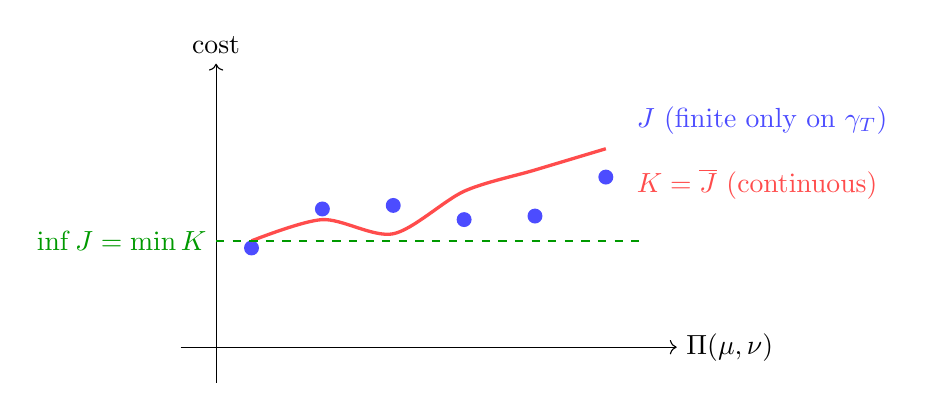
\begin{tikzpicture}[scale=0.9]
    % Axes
    \draw[->] (-0.5, 0) -- (6.5, 0) node[right] {$\Pi(\mu, \nu)$};
    \draw[->] (0, -0.5) -- (0, 4) node[above] {cost};

    % J (only finite at discrete points)
    \foreach \x in {0.5, 1.5, 2.5, 3.5, 4.5, 5.5} {
        \pgfmathsetmacro{\y}{1 + 0.5*sin(\x*60) + 0.3*\x}
        \fill[blue!70] (\x, \y) circle (3pt);
    }
    \node[blue!70, right] at (5.8, 3.2) {$J$ (finite only on $\gamma_T$)};

    % K (continuous extension)
    \draw[red!70, very thick, smooth] plot coordinates {(0.5, 1.5) (1.5, 1.8) (2.5, 1.6) (3.5, 2.2) (4.5, 2.5) (5.5, 2.8)};
    \node[red!70, right] at (5.8, 2.3) {$K = \overline{J}$ (continuous)};

    % Infimum line
    \draw[green!60!black, dashed, thick] (0, 1.5) -- (6, 1.5);
    \node[green!60!black, left] at (0, 1.5) {$\inf J = \min K$};
\end{tikzpicture}
\end{center}

\textbf{Key insight:}
\begin{itemize}
    \item $J$ is only finite on the ``discrete'' set $\{\gamma_T\}$
    \item $K$ is the continuous envelope
    \item Both have the same infimum!
\end{itemize}
\end{frame}

%==============================================================================
\begin{frame}{Exercise: Relaxation Application}
\begin{block}{Exercise}
Recall the three segments example from 1-4.tex:
\begin{itemize}
    \item Segments $A$ (at $x=0$), $B$ (at $x=1$), $C$ (at $x=-1$)
    \item $\mu = \Hone \llcorner A$, $\nu = \frac{1}{2}(\Hone \llcorner B + \Hone \llcorner C)$
\end{itemize}
\begin{enumerate}
    \item[(a)] We showed $\inf_{\text{maps}} M(T) = 1$ but no optimal map exists. Why?
    \item[(b)] Theorem 1.33 says $\inf J = \min K$. What is $\min K$?
    \item[(c)] What is the optimal plan $\gamma^*$ achieving $\min K$?
\end{enumerate}
\end{block}
\end{frame}

%==============================================================================
\begin{frame}{Solution: Relaxation Application}
\textbf{(a)} Why no optimal map exists:
\begin{itemize}
    \item To achieve cost $= 1$: all points must move purely horizontally
    \item But then either all go to $B$ or all go to $C$
    \item Cannot satisfy $\nu = \frac{1}{2}(\Hone \llcorner B + \Hone \llcorner C)$!
\end{itemize}

\vspace{0.3cm}
\textbf{(b)} By Theorem 1.33:
\[
\min K = \inf J = 1
\]

\vspace{0.3cm}
\textbf{(c)} The optimal plan:
\[
\boxed{\gamma^* = \frac{1}{2}\gamma_{T^+} + \frac{1}{2}\gamma_{T^-}}
\]
where $T^\pm(x) = x \pm e$, $e = (1, 0)$.
\begin{itemize}
    \item NOT map-induced (convex combination of two map-induced plans)
    \item But it IS the weak limit of $\gamma_{T_n}$
    \item $K(\gamma^*) = 1$ = minimum!
\end{itemize}
\end{frame}

%==============================================================================
\section{Convex Functions}
%==============================================================================

\begin{frame}{Box 1.11: Convex Functions Memo}
\begin{block}{Definition}
$f : \R^d \to \R \cup \{+\infty\}$ is \textbf{convex} if for all $x, y \in \R^d$ and $t \in [0,1]$:
\[
f((1-t)x + ty) \leq (1-t)f(x) + tf(y)
\]
\end{block}

\vspace{0.3cm}
\textbf{Equivalent characterization:} The \textbf{epigraph}
\[
\text{epi}(f) = \{(x, z) \in \R^d \times \R : z \geq f(x)\}
\]
is a convex set.

\begin{center}
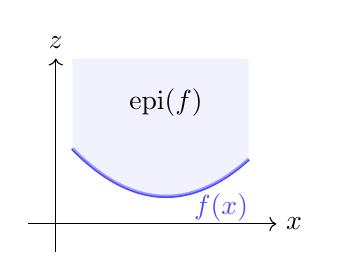
\begin{tikzpicture}[scale=0.7]
    \draw[->] (-0.5, 0) -- (4, 0) node[right] {$x$};
    \draw[->] (0, -0.5) -- (0, 3) node[above] {$z$};

    % Convex function
    \draw[blue!70, very thick] plot[smooth, domain=0.3:3.5] (\x, {0.3*(\x-2)^2 + 0.5});

    % Epigraph shading
    \fill[blue!10, opacity=0.5] plot[smooth, domain=0.3:3.5] (\x, {0.3*(\x-2)^2 + 0.5}) -- (3.5, 3) -- (0.3, 3) -- cycle;

    \node[blue!70] at (3, 0.3) {$f(x)$};
    \node at (2, 2.2) {epi$(f)$};
\end{tikzpicture}
\end{center}
\end{frame}

%==============================================================================
\begin{frame}{Stability: Supremum of Convex Functions}
\begin{block}{Proposition}
If $\{f_\alpha\}_{\alpha \in A}$ is a family of convex functions, then:
\[
f(x) := \sup_{\alpha \in A} f_\alpha(x)
\]
is also convex.
\end{block}

\vspace{0.3cm}
\textbf{Proof 1 (direct):}
\[
f_\alpha((1-t)x + ty) \leq (1-t)f_\alpha(x) + tf_\alpha(y) \leq (1-t)f(x) + tf(y)
\]
Pass to $\sup$ in $\alpha$: $f((1-t)x + ty) \leq (1-t)f(x) + tf(y)$. \checkmark

\vspace{0.3cm}
\textbf{Proof 2 (epigraph):}
\[
\text{epi}(f) = \bigcap_{\alpha} \text{epi}(f_\alpha)
\]
Intersection of convex sets is convex. \checkmark
\end{frame}

%==============================================================================
\begin{frame}{Exercise: Convex Functions}
\begin{block}{Exercise}
Determine if each function is convex:
\begin{enumerate}
    \item[(a)] $f(x) = |x|^2$ on $\R$
    \item[(b)] $f(x) = \max(0, x)$ on $\R$
    \item[(c)] $f(x) = -\sqrt{x}$ on $[0, \infty)$
    \item[(d)] $f(x) = x^3$ on $\R$
\end{enumerate}
\end{block}

\vspace{0.3cm}
\textit{Hint:} For smooth functions, $f'' \geq 0$ characterizes convexity.
\end{frame}

%==============================================================================
\begin{frame}{Solution: Convex Functions}
\textbf{(a)} $f(x) = x^2$: \quad $f''(x) = 2 > 0$ \quad $\Rightarrow$ \textbf{Convex} \checkmark

\vspace{0.3cm}
\textbf{(b)} $f(x) = \max(0, x)$:
\begin{itemize}
    \item $f = \sup(0, \text{id})$, supremum of two affine (hence convex) functions
    \item $\Rightarrow$ \textbf{Convex} \checkmark
\end{itemize}

\vspace{0.3cm}
\textbf{(c)} $f(x) = -\sqrt{x}$ on $[0, \infty)$:
\begin{itemize}
    \item $f'(x) = -\frac{1}{2\sqrt{x}}$, \quad $f''(x) = \frac{1}{4x^{3/2}} > 0$
    \item $\Rightarrow$ \textbf{Convex} \checkmark
\end{itemize}

\vspace{0.3cm}
\textbf{(d)} $f(x) = x^3$ on $\R$:
\begin{itemize}
    \item $f''(x) = 6x$: positive for $x > 0$, negative for $x < 0$
    \item $\Rightarrow$ \textbf{NOT convex} on $\R$ (but convex on $[0, \infty)$)
\end{itemize}
\end{frame}

%==============================================================================
\begin{frame}{Visualization: $x^3$ is Not Convex}
\begin{center}
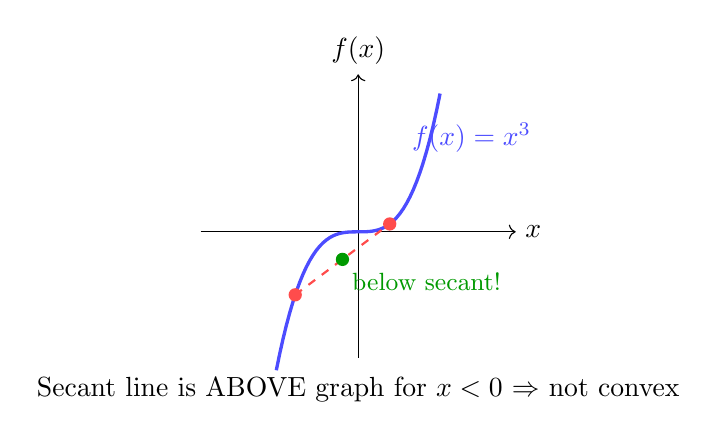
\begin{tikzpicture}[scale=0.8]
    \draw[->] (-2.5, 0) -- (2.5, 0) node[right] {$x$};
    \draw[->] (0, -2) -- (0, 2.5) node[above] {$f(x)$};

    % f(x) = x^3
    \draw[blue!70, very thick, domain=-1.3:1.3, samples=50] plot (\x, {\x*\x*\x});

    % Secant line showing non-convexity
    \draw[red!70, thick, dashed] (-1, -1) -- (0.5, 0.125);

    % Points
    \fill[red!70] (-1, -1) circle (3pt);
    \fill[red!70] (0.5, 0.125) circle (3pt);

    % Midpoint
    \fill[green!60!black] (-0.25, -0.4375) circle (3pt);
    \node[green!60!black, below right, font=\small] at (-0.25, -0.5) {below secant!};

    \node[blue!70] at (1.8, 1.5) {$f(x) = x^3$};

    % Caption
    \node at (0, -2.5) {Secant line is ABOVE graph for $x < 0$ $\Rightarrow$ not convex};
\end{tikzpicture}
\end{center}
\end{frame}

%==============================================================================
\section{Summary}
%==============================================================================

\begin{frame}{Summary}
\textbf{Transport Map Existence:}
\begin{itemize}
    \item \textbf{Lemma 1.27:} $\mu$ atomless on $\R$ $\Rightarrow$ $\exists T$ with $T_\# \mu = \nu$
    \item \textbf{Lemma 1.28:} Borel bijection $\sigma_d : \R^d \leftrightarrow \R$ (decimal interleaving)
    \item \textbf{Corollary 1.29:} $\mu$ atomless on $\R^d$ $\Rightarrow$ $\exists T$ with $T_\# \mu = \nu$
\end{itemize}

\vspace{0.3cm}
\textbf{Density and Relaxation:}
\begin{itemize}
    \item \textbf{Lemma 1.31:} Same mass on partition cells $\Rightarrow$ weak convergence
    \item \textbf{Theorem 1.32:} $\{\gamma_T\}$ is \textbf{dense} in $\Pi(\mu, \nu)$ when $\mu$ atomless
    \item \textbf{Theorem 1.33:} $K = \overline{J}$ (relaxation), so $\boxed{\inf J = \min K}$
\end{itemize}

\vspace{0.3cm}
\textbf{Convex Functions:}
\begin{itemize}
    \item Supremum of convex functions is convex
    \item Key tool for \textbf{c-concavity} (next lecture)
\end{itemize}
\end{frame}

\end{document}
